\documentclass{article}

\makeatletter
\newif\ifhtlatex
\@ifpackageloaded{tex4ht}{\htlatextrue}{\htlatexfalse}
\makeatother

\usepackage{amsmath}
\usepackage[margin=0.93in]{geometry}
\usepackage{graphicx}
\usepackage{calc}

\usepackage{hyperref}
\hypersetup{colorlinks=false,pdfborder={0 0 0}}

\def\name{Peter B.~Denton, Ph.D.}
\title{CV}

\pagestyle{myheadings}
\markright{\name}
\thispagestyle{empty}

\usepackage{sectsty}
\sectionfont{\rmfamily\mdseries\Large}
\subsectionfont{\rmfamily\mdseries\itshape\large}
\subsubsectionfont{\rmfamily\mdseries\itshape\normalsize}

\setlength\parindent{0em}

\renewenvironment{itemize}{
\begin{list}{}{
\setlength{\leftmargin}{.5em}}}{
\end{list}}

\begin{document}

\ifhtlatex
\Tag{TITLE+}{CV}
\fi

% % % % % With headshot
% 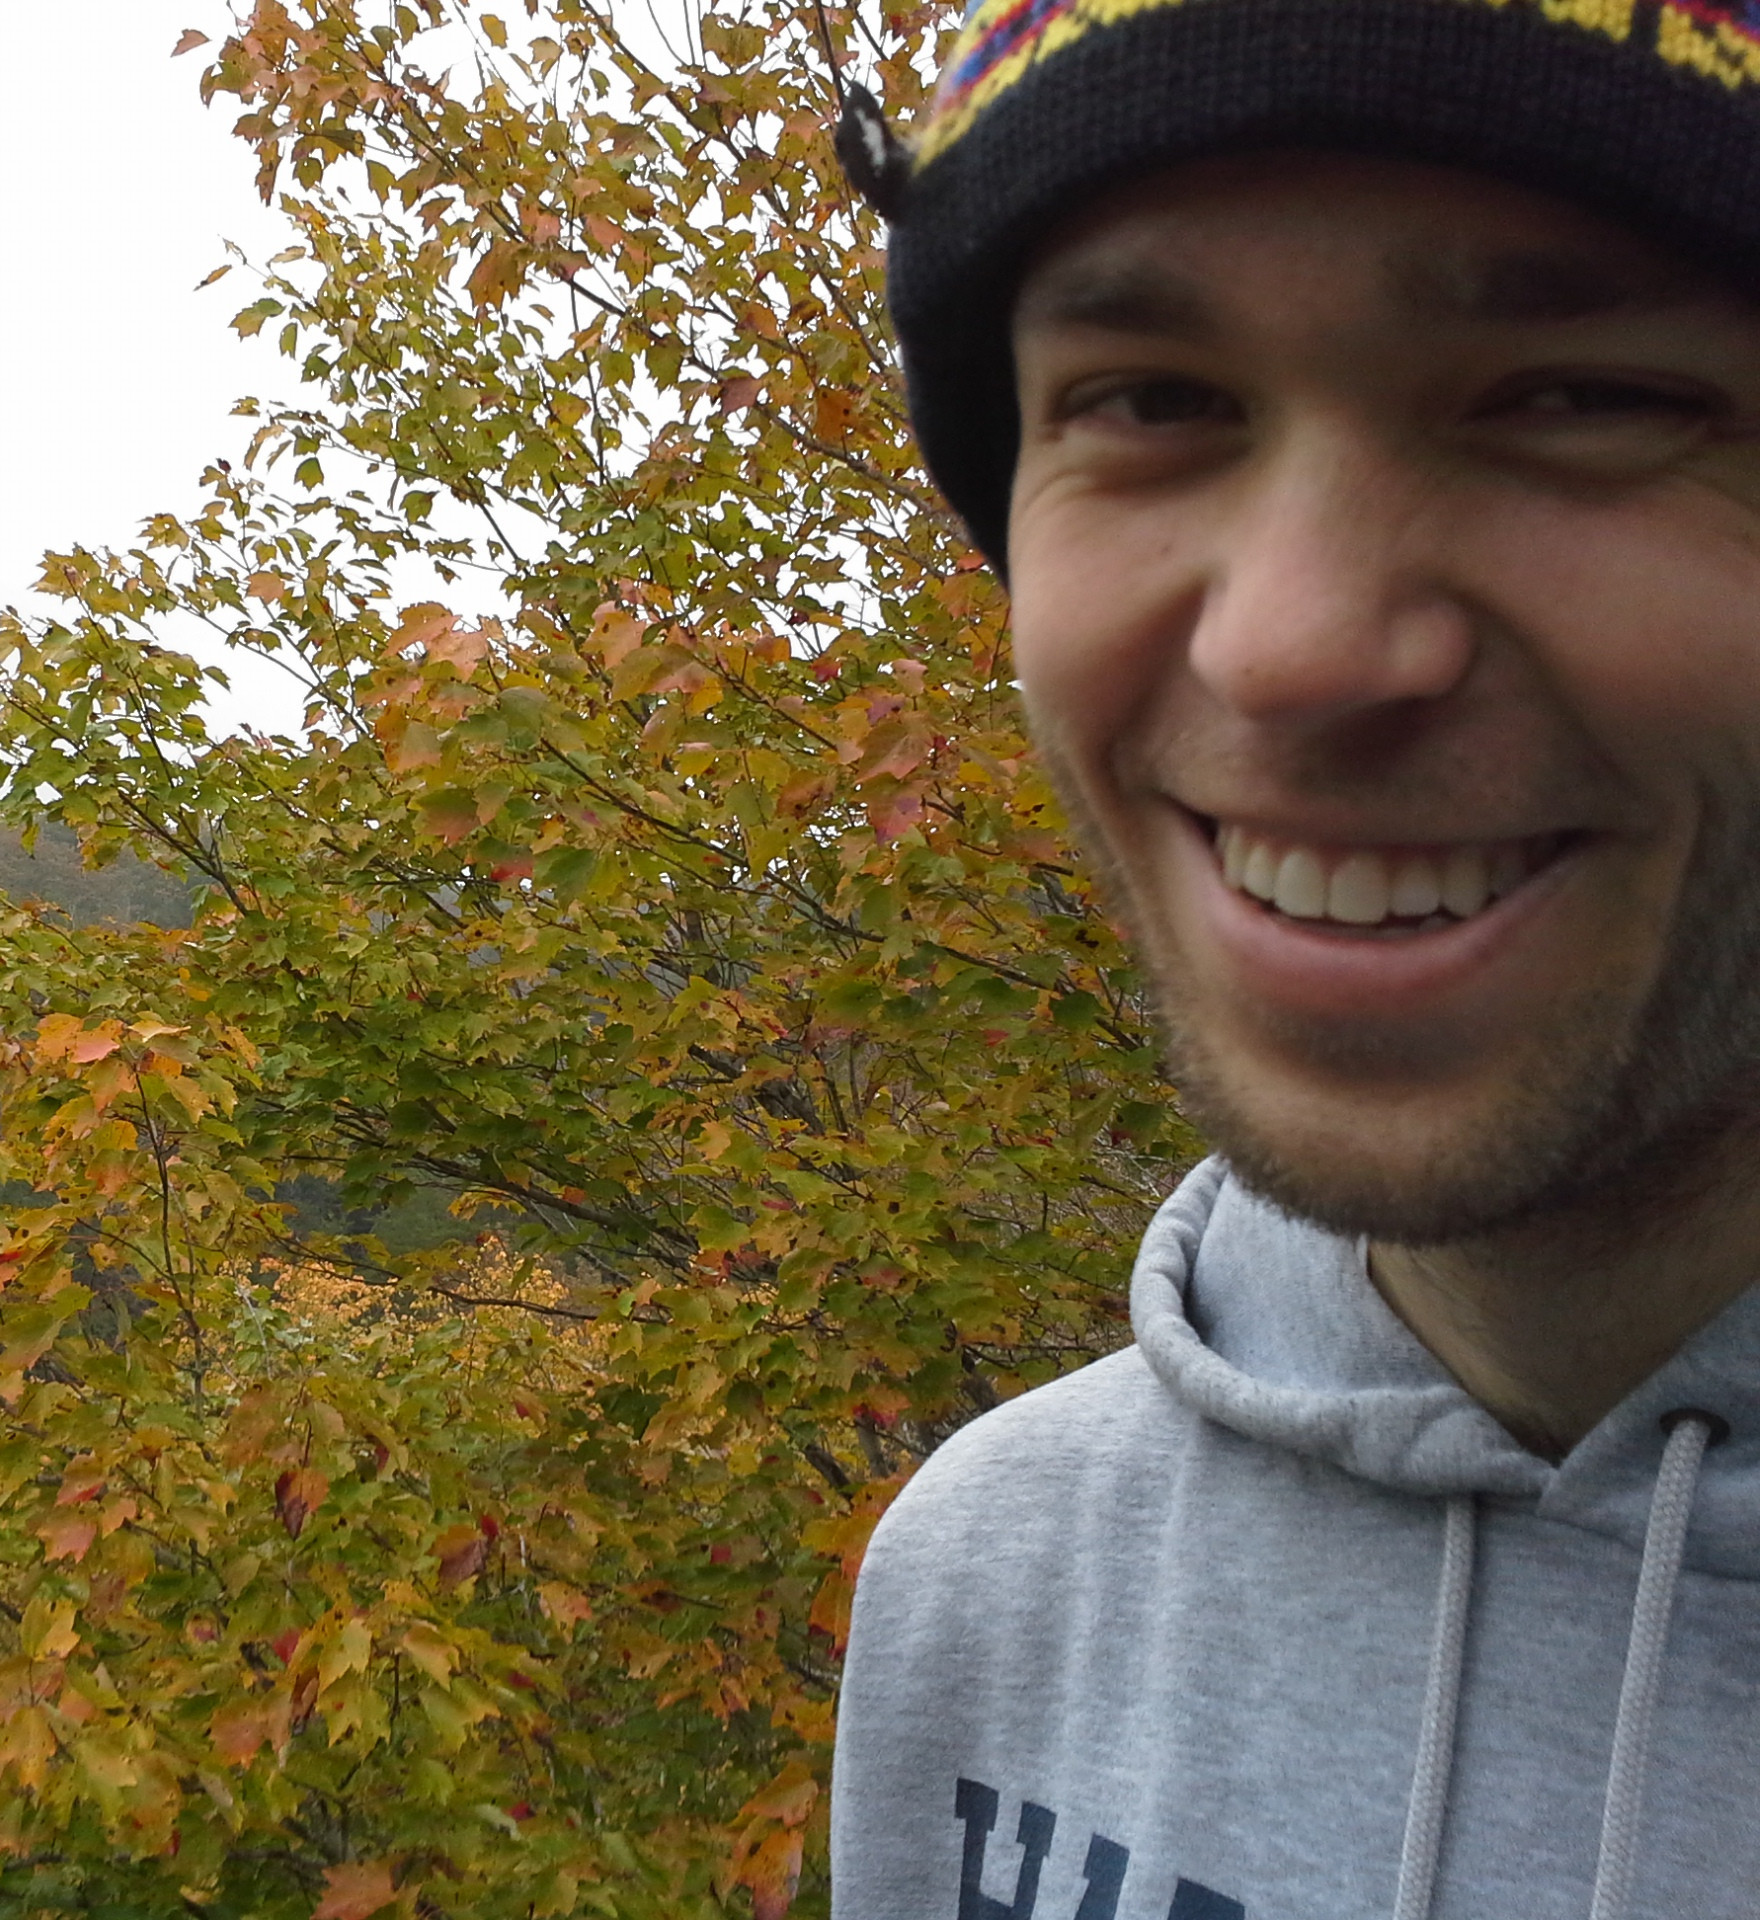
\includegraphics[width=1.2in]{face_cropped}
% \parbox{\textwidth-1.3in}{\vspace*{-1.1in}
% {\huge \name}\\
% \vspace*{0.1in}
% \begin{tabular}{ll|l|ll}
% +45 71 49 29 40 & Gernersgade 35, 1 th & Updated: & \today\\
% \href{mailto:peterbd1@gmail.com}{\tt peterbd1@gmail.com} & Copenhagen K 1319 & Website: & 
% \href{http://peterdenton.github.io}{\tt peterdenton.github.io}
% \end{tabular}
% }

% % % % % Without headshot
\vspace*{-0.5in}
{\huge \name}\hfill\includegraphics[height=0.8in]{BNL}\\
\vspace{0.1in}
\begin{tabular}{ll|l|ll}
Phone: & +1-631-344-3767 & Bldg 510A PO Box 5000 & Updated: & \today\\
Email: & \href{mailto:peterbd1@gmail.com}{\tt peterbd1@gmail.com} & Upton, NY 11973 & Website: & 
\href{http://peterdenton.github.io}{\tt peterdenton.github.io}
\end{tabular}

\subsection*{Research Experience}
\begin{itemize}
\item Assistant Physicist at Brookhaven National Laboratory, October 2018--Present.
\item Postdoctoral Fellow with Irene Tamborra at Niels Bohr International Academy, September 2016--August 2018.
\item Graduate Student Research Program in Theoretical Physics with Stephen Parke at Fermilab, August 2015--August 2016.
\item DOE funded research assistant with Thomas J.~Weiler at Vanderbilt University, Spring 2011--Fall 2015.
\item Research assistant with Sokrates Pantelides at Vanderbilt University, Summer--Fall 2010.
\item Lee Teng Internship with Tanaji Sen at Fermilab, Summer 2009.
\item Bonner Labs with Bill Llope at Rice University, Summer 2008.
\end{itemize}

\subsection*{Research Interests}
\begin{itemize}
\item SM and BSM neutrino theory.
\item Astroparticle physics.
\end{itemize}

\subsection*{Education}
\begin{itemize}
\item Ph.D.~Physics, Vanderbilt University, August 2016.
\item B.S.~Physics, Rice University, May 2010.
\item B.A.~Mathematics, Rice University, May 2010.
% \item Multi-variable calculus, differential equations, Grand Rapids Community College, 2005--2006.
\end{itemize}

\subsection*{Honors and Awards}
\begin{itemize}
\item Neutrino Physics Center (NPC) award of \$10,000 to work with Stephen Parke at Fermilab, awarded December 2018.
\item Neutrino Theory Network (NTN) award of \$14,000 to work with Irina Mocioiu at PSU, awarded June 2018.
\item The Giorgio Salvini diploma from the Erice International School of Subnuclear Physics, awarded June 2016.
\item PITT PACC travel award to attend Pheno '16, awarded April 2016.
\item Vanderbilt Dissertation Enhancement Grant of \$2,000 to attend the Theoretical Advanced Study Institute, awarded April 2014.
\item Subsidy of \$1,600 to attend the Theoretical Advanced Study Institute: Amplitudes For Colliders in June 2014, awarded April 2014.
\item Division of Particles \& Fields travel grant to the APS April 2013 meeting, awarded March 2013.
\item The Robert T.~Lagemann Award of \$1,000 for highest academic achievement by a first-year graduate student, awarded April 2011.
\item McMinn Fellowship of \$25,000 over five years, awarded March 2010.
\end{itemize}

\subsection*{Collaborations}
\begin{itemize}
\item Giant Radio Array for Neutrino Detection (GRAND), 2017--Present.
\end{itemize}

\subsection*{Physics Schools}
\begin{itemize}
\item Erice International School of Subnuclear Physics in Sicily (ISSP), June 2016.
\item Theoretical Advanced Study Institute in Elementary Particle Physics (TASI), Boulder CO, June 2014.
\item Introduction to accelerator physics, United States Particle Accelerator School, June 2009.
\end{itemize}

\subsection*{Software}
\begin{itemize}
\item 
c++, mpi, openmp, python, matplotlib, \LaTeX, beamer, GLoBES, pythia, ROOT, MATHEMATICA, MATLAB, FORTRAN, gnuplot, java, html, javascript, \dots
\end{itemize}

\subsection*{Service}
\begin{itemize}
\item Snowmass neutrino oscillations subtopic convener and neutrino theory liason 2020--2021.
\item International Organizing Committee for Neutrino 2020.
\item Convener for Brookhaven Forum 2019 and DPF 2019.
\item Judge for the 12th International Neutrino Summer School at Fermilab 2019. 
\item Chair for Pheno 2019, 2020.
\item Reviewer for Physical Review Letters, Journal of High Energy Physics, Physical Review D, Physics Letters B, European Physical Journal C, Journal of Mathematical Physics, Nuclear Physics B, Monthly Notices of the Royal Astronomical Society, and Universe.
\item Brookhaven Neutrino Theory Virtual Seminar creator/organizer, 2020--Present.
\item BNL HET seminar organizer, 2019--Present.
\item BNL HET lunch discussion organizer, 2019--Present.
\item NBIA Astroparticle journal club co-chair, 2017--2018.
\end{itemize}

\subsection*{Outreach}
\begin{itemize}
\item Interact with grade-school students via APS's \emph{Adopt-A-Physicist}, Skype-A-Scientist, $\dots$ programs, 2018--Present.
\item Brookhaven Women In Science (BWIS) member, 2020--Present.
\end{itemize}

\subsection*{Students Advised/Mentored}
\begin{itemize}
\item Klaes M\o ller, University of Copenhagen, master's thesis: \emph{Constraining Astrophysical Parameters with Neutrinos}, 2017--2018.
\item Anna Suliga, University of Copenhagen, master's thesis: \emph{Diffuse supernova neutrino background}, 2017--2018.
Currently PhD student at University of Copenhagen.
\item Mia-Louise Nielsen, University of Copenhagen, bachelor's thesis: \emph{Star-forming galaxies as sources of high energy neutrinos}, 2017.
Currently masters student at University of Copenhagen.
\end{itemize}

\subsection*{Teaching}
\begin{itemize}
\item Teaching assistant at Vanderbilt University, Fall 2010--Spring 2015.
\item Teaching assistant for the Physics Department at Rice University, Fall 2009.
\item Writing consultant at Rice University, 2007--2010.
\item Tutoring English, math, and physics at middle school, high school, undergraduate, and graduate school levels, 2005--2015.
\end{itemize}

\subsection*{Professional Societies}
\begin{itemize}
\item Member, American Physical Society.
\end{itemize}

\end{document}
